\feelchapter{Heat sink}
            {Heat sink}
            {Baptiste Morin, Christophe Prud'homme}
            {cha:thermalfin}

This problem considers the performance of a heat sink designed for the thermal management of high-density electronic components. The heat sink is comprised of a base/spreader which in turn supports a number of plate fins exposed to flowing air. We model the flowing air through a simple convection heat transfer coefficient. From the engineering point of view, this Problem illustrates the application of conduction analysis to an important class of cooling problems: electronic components and systems. \\ \\
Our interest is in the conduction temperature distribution at the base of the spreader. The target is to study how the heat transfer occures with different parameters on our heat sink. The heat generated by high-density electronic components is such that it's very expensive to cool large structures (data center). The cooling optimization is consequent in the run for decreasing operating costs.

\noindent A classical thermal CPU cooler looks like this 

\begin{figure}[!h]
\centering
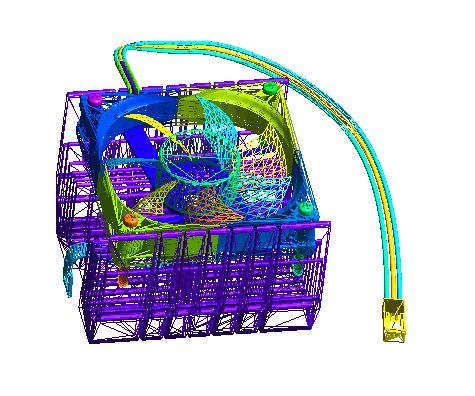
\includegraphics[width=.45\linewidth]{heatsink/complete_cooler.png}
\caption{Mesh of a classic CPU cooler}
\end{figure}

\noindent We are here going to describe how it is theorically working and how it is impleted with \feel. 

\section{Problem description}
\subsection{Domain}

We consider here a classical "radiator" which is a CPU heat sink. Those types of coolers are composed with a certain number of plate fins exposed to flowing air or exposed to a ventilator. Regarding the periodicity and geometry of our concern, we can make our study on a characteristic element of the problem : a half cell of the heat sink single thermal fin with its spreader at the basis. Let's take a look at the geometry of our problem :

\begin{figure}[!h]
\centering
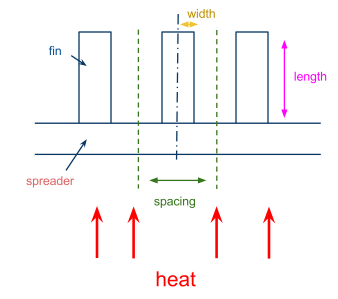
\includegraphics[width=.45\linewidth]{heatsink/sink_geom.png}
\caption{Geometry of heat sink}
\end{figure}

Our study is avaible in 2 or 3 dimensions, depending on the application's parameters. You'll see later how to work with it. Let's see on which meshes we are working on :
\begin{figure}[!h]
\begin{minipage}[b]{.50\linewidth}
\centering
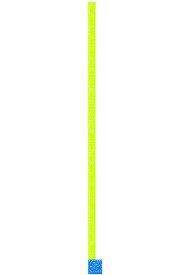
\includegraphics[width=.45\linewidth]{heatsink/mesh_2d.png}
\caption{2D mesh}
\end{minipage}
\begin{minipage}[b]{.50\linewidth}
\centering
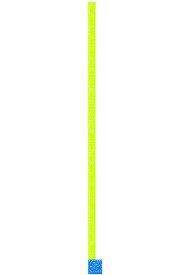
\includegraphics[width=.45\linewidth]{heatsink/mesh_2d.png}
\caption{3D mesh}
\end{minipage}
\end{figure}

We consider the physical domain $\varOmega (\mu)$ where $\mu = (\mu_1, ...,\mu_p)$ represents the parameters of our concern. 

\subsection{Domain parameters}
We are here only talking about the domain parameters of $\varOmega(\mu)$ which will define our half cell. Furthers parameters are also avaible but are described in ~\ref{therm:param}.


\subsubsection{Biot number}
The Biot number $Bi$ is a dimensionless number used in non-steady or transient states in heat transfer calculations. It gives a simple index of the ratio of the heat transfer resistances inside  and at the surface of a body. This number determines wheter or not the temperatures insdide a body will significantly vary in space while the body heats or cools over time from a thermal gradient applied to its surface. This number is defined as 
\begin{equation}
Bi = \frac{hL_c}{k_b}
\end{equation} 
where $h$ is the heat transfert coefficient, $L_c$ is the characteristic length (commonly defined as the volume of the body divided by the surface area) and $k_b$ is the thermal conductivity of the body. 

\subsubsection{Material}

Here the material parameter can be described with the spreader-to-fin conductivity ratio $\kappa$.

\subsubsection{Spacing}
This parameter represents the length between two plates fin.

\subsubsection{Thickness}
The thickness of a platefin (divied by two here because we are working on a half cell).

\subsubsection{Width}

This parameter is to take into account only if you are considering the 3D issue. Typically, this parameter is linked with constructor's standards. We have chosen here to work with one of the well-known : Intel. 


\section{Theory and implementation}
\subsection{Equations}

\subsubsection{Steady-state}
Here the steady state can be considered as the standard state because it corresponds to the standard utilisation of the components. This state satisfies the conduction equation.

\subsubsection{Transient states}


\subsection{Boundary conditions}
The problem requieres that the temperature and heat flux are continute on fin or spreader interfaces. Considering the problem's geometry, we also impose zero heat flux on the vertical surfaces of the spreader. 

\section{Application parameters}
\label{therm:param}


